\chapter{CAHIER DES CHARGES}


\section{EXPRESSION DES BESOINS}
Une fois le système conçu et déployé il sera accessible aux utilisateurs de la plateforme avec des niveaux d’accès selon les différents profils qui sont énoncés dans les points qui suivent. Ces besoins connus et définis sont groupés en deux types de besoins.


 \subsection{BESOINS FONCTIONNELS}
 
 Les besoins fonctionnels désignent les fonctions que le produit fini doit posséder pour qu’il soit considéré comme fonctionnel. Dans le cas de notre Data Warehouse, pour les profiles suivant il doit pouvoir :
 
 \textbf{Pour le profile administrateur}, on retrouve les exigences suivantes : 
 \begin{itemize}
\item Fournir un tableau de bord accessible en ligne qui permettra de renseigner l’administrateur sur :
\begin{list}{•}{ }
   \item L’activité des réservations sur des périodes modulable selon le grée de l’utilisateur sur les  années, les trimestres et les mois passé et en cours
   \item L’activité des hôteliers sur les mêmes périodicités que le point précédent. Ici il s’agira des détails tel que le chiffre d’affaire de chaque hôtelier le nombre de nuitées, le nombre de chambres réservés et les paiements mensuels de ce dernier.
   \item L’activité des utilisateurs en général. On fournira comme informations le nombre de visites par jour, par mois, par trimestre et par années.
   \item Les différentes offres de la plateforme et leurs appréciations dans le temps.

\end{list}

   \item Fournir un système accessible sur le serveur de l’entreprise qui aura un tableau de bord similaire à 
celui en ligne avec des fonctionnalités en plus. On aura les fonctionnalités suivant :
\begin{list}{•}{ }
   \item Intégrer aux informations de réservations des informations de météo du lieu de provenance de la personne qui réserve et celui de l’endroit où l’hôtel de destination grâce à un service de météo en ligne qui sera utilisé comme source de données.
   \item Un comparatif de la liste d’hôtel issue du site du ministère du tourisme Camerounais. Ces informations seront reçu dans un fichier Excel et devra être utilisé comme source de données\\
\end{list}
 
 \end{itemize}
 
\textbf{Pour le profile Hôtelier}, On dégage les fonctionnalités suivantes : 
   \begin{list}{•}{ }
   \item Un tableau de bord permettant a l’utilisateur de suivre les réservations émises pour son établissement, les tendances de ses offres et promotions, les chambres les plus prisées et le chiffre d’affaire. Ces informations seront disponibles en temps réel et on pourra consulter l’historique de ces informations.
   \item Des indicateurs de performances qui seront disposé en temps réel sur le profil de l’utilisateur et qui reflètent l’activité hebdomadaire ou mensuelle.
Pour le profile client on devra fournir :
   \item Sur son profile on devra afficher des indicateurs de son activité et des graphes qui permet de visualiser le chiffre d’affaire qu’il génère sur une période d'un an.
Tous ces besoins ont été apprécié et pourront évoluer d’où le besoin fondamentale de développer une solution apte à subir des maintenances évolutives et correctives sans avoir à détruire ou recommencer ce qui a été fait.
\end{list}



 \subsection{BESOINS NON FONCTIONNELS}
 
 Les besoins non fonctionnels désignent les conditions à remplir pour qu’une solution logicielle fonctionne correctement. Dans le cas de notre application, ces conditions doivent être remplir :
 \begin{list}{•}{ }
 \item Un serveur de base de données pour stocker les données du data warehouse.
 \item Un une connexion internet pour exploiter les sources de données qui sont pour la majorité des API en ligne.\\
 \end{list}


L'ensemble des besoins énuméré plus constitue une partie des questionnements qui feront du data warehouse  un produit fonctionnel et exploitable par l’ensemble des décideurs de la plateforme Hosteline.

 \cleardoublepage
 \section{CONTRAINTES LIÉES AU PROJET}
 
 Les contraintes sont l’ensemble de la (définition). Pour ce projet nous avons fait face a des contrainte de de différentes nature que nous avons regroupé sous les points qui suivant.\\
 
 \subsection{EXIGENCES DE DOCUMENTATION}
 
 En effet la solution une fois développé et déployé devra être appuie d’une forte documentation pour les utilisateurs et les développeurs qui prendrons le relais dans la maintenance de la solution. Un manuel d’utilisateur devra être fournis pour chacun des profils utilisateur de la solution et sera accessible en un clic sur les diffèrent profiles du système selon le niveau d’accès et les fonctionnalités. Aussi un document contenant les détails de d’implémentation et de déploiement de la solution sera fourni et mis à la disposition de l’équipe de développement en charge de maintenir et faire évoluer la solution. Pour une assistance à l’utilisateur une FAQ (Foire aux questions) sera intégré au site web ou un sous domaine du site pour faciliter la prise en main par les utilisateurs de la solution.\\
 
 \subsection{EXIGENCES DE QUALITÉ}
 
 Le but de la mise en œuvre de ce système décisionnel est l’augmentation du chiffre d’affaire de Hosteline passant par une meilleure qualité de service. La solution elle-même devra respecter des standards de qualité qui correspondent à ce type de projet.\\
 
 
 \subsection{CONTRAINTES TEMPORELLES}
 
 Cette contrainte s’est avérer être la plus difficile à respecter car l’équipe en charge du projet manquais d’expérience dans la mise en œuvre de solution décisionnel. Néanmoins avec un redoublement d’effort on a pu réduire le retard à juste un mois. On est passé de quatre mois que prévoyais le calendrier de départ a cinq mois. Le diagramme de gant de la figure XX présente le planning prévisionnel qui a été fixé au départ avec une équipe de trois développeurs. 
 
 \subsection{CONTRAINTES MATÉRIEL ET LOGICIEL}
 
 Pour la mise en place du système on a du se munir d’un matériel spécifique remplissent des conditions qui doivent satisfaire les exigences de vitesse et mémoire du système. Parmi ce matériel on a dénombré : 
 \begin{list}{•}{ }
   \item Une machine qui fera office de serveur local avec de caractéristiques minimal de 4Giga de ram, un processeur2.6 Core I3, 300 Giga de ROM avec un système d’exploitation Windows 7 ou plus.
   \item Le logiciel Pentaho de préférence dans sa dernière version (8.1.0 lors de la rédaction de ce mémoire)\\
 \end{list}

   
 \section{DÉMARCHE DE RÉALISATION}
 \subsection{INTERVENANTS DU PROJET}
 Ce qui fait en générale l’intérêt d’un projet c’est sa capacité à résoudre le problème d’un ensemble de personnes. Ainsi la pertinence du projet dépend au finale du niveau de satisfaction que peut offrir le produit fini aux parties prenantes de l’effort. Les intervenants dans un projet c’est l’ensemble des personnes qui de près ou de loin influencent le déroulement du projet. La mise en place du système décisionnel de Hosteline a comme parties prenantes :
 \begin{list}{•}{ }
   \item Les propriétaires d’établissement hôteliers et clients hôteliers de Hosteline,
   \item Les clients qui viennent réserver des logements sur la plateforme
   \item Les promoteurs de la plateforme Hosteline
   \item L’équipe de développement\\
 \end{list}

Toutes ces groupes de personnes ci-dessus sont celles qui ont eu un apport considérable a la bonne marche du projet et sans elles ce projet n’aurait pas tout son sens car le but était de satisfaire ces parties prenantes d’une manière ou d’une autre.

 \subsection{PLANIFICATION DU PROJET}
 
 Pour garantir le bon déroulement du projet, tout en respectant les délais, élaboré une planification globale de conduite du projet. Le diagramme suivant décrit cette planification ainsi que l’ordonnancement prévu des phases du projet. 
 \subsection{DIAGRAMME DE GANTT }
 
  Le diagramme de Gantt, couramment utilisé en gestion de projet, est l’un des outils les plus efficaces pour représenter visuellement l’état d’avancement des différentes activités (tâches) qui constituent un projet. La colonne de gauche du diagramme énumère toutes les tâches à effectuer, tandis que la ligne d’en-tête représente les unités de temps les plus adaptées au projet (jours, semaines, mois etc.). Chaque tâche est matérialisée par une barre horizontale, dont la position et la longueur représentent la date de début, la durée et la date de fin. Ce diagramme permet donc de visualiser d’un seul coup d’œil :
  \begin{list}{•}{ }
   \item Les différentes tâches à envisager
   \item La date de début et la date de fin de chaque tâche
   \item La durée escomptée de chaque tâche
   \item Le chevauchement éventuel des tâches, et la durée de ce chevauchement
   \item La date de début et la date de fin du projet dans son ensemble\\
  \end{list}

\begin{figure}[!htbp]
	\begin{center}
		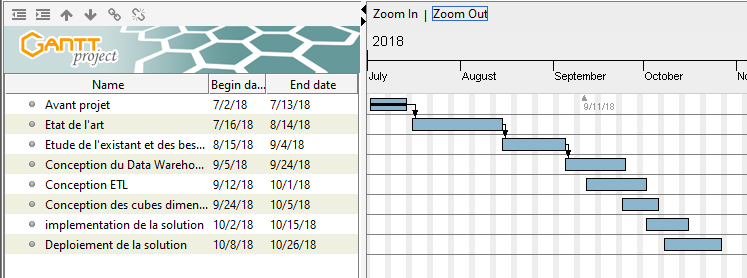
\includegraphics[scale=0.85]{images/gantt.png}
		\caption{Diagramme de GANTT.}
		\label{use_bi_tools}
	\end{center}
\end{figure}

  %\section{CALENDRIER PRÉVISIONNEL}
  
  %\subsection{CHRONOGRAMME}
 % \subsection{ESTIMATION DU COUT DE LA SOLUTION}
  
 % \textbf{RESSOURCES HUMAINES}\\
 %	Pour chaque phase du projet nous avons fait appel à des compétences divers dans le domaine du décisionnel. Ces rôles ont été jouées en majorité par notre petite équipe de quatre développeurs mais les compétences exploité à chaque niveau étais différemment apprécié et rémunéré. Le tableau suivant récapitule.\\

 % \textbf{RESSOURCES MATERIELS}\\

